\documentclass[conference]{IEEEtran}
\IEEEoverridecommandlockouts
% The preceding line is only needed to identify funding in the first footnote. If that is unneeded, please comment it out.
\usepackage{cite}
\usepackage{amsmath,amssymb,amsfonts}
\usepackage{algorithmic}
\usepackage{graphicx}
\usepackage{textcomp}
\def\BibTeX{{\rm B\kern-.05em{\sc i\kern-.025em b}\kern-.08em
    T\kern-.1667em\lower.7ex\hbox{E}\kern-.125emX}}
\begin{document}

\title{Enhancing performance and reliability of Network File System\\
}

\author{
\makebox[.5\linewidth]{ Aswin Babu Karuvally }\\
Department of Computer Applications \\
College of Engineering Trivandrum, KTU\\
Trivandrum, Kerala \\
aswinbabuk@gmail.com\\
\and \makebox[.5\linewidth]{ Basith Hameem }\\
Department of Computer Applications \\
College of Engineering Trivandrum, KTU\\
Trivandrum, Kerala \\
basithhameem@cet.ac.in\\
\and \makebox[.5\linewidth]{Ann Jerin Sundar }\\
Department of Computer Applications \\
College of Engineering Trivandrum, KTU\\
Trivandrum, Kerala  \\
annjerinajs@gmail.com\\
\and \makebox[.5\linewidth]{Prof. John Prakash Joseph}\\
Asst. Professor, Department of Computer Applications \\
College of Engineering Trivandrum, KTU\\
Trivandrum, Kerala \\
john@cet.ac.in\\
\\
}
\maketitle

\begin{abstract}
Network File System is a widely used distributed file system that allows the
user to access and manipulate storage on remote computers, as if they were a
part of the local machine. Network File System is notoriously slow in its 
default configuration and the incorporation of more than a dozen clients in the 
NFS environment merely accentuates the delay. When configured to deliver faster
speeds by turning on asynchronous mode, the system suffers from higher risk of 
data corruption and loss.

This study proposes variegated modifications to the Network File System,
enabling it to provide elevated system performance, while containing
the risk of data loss and corruption. Further, the proposed system behaves
better in congested networks by consuming less bandwidth, ensuring decent
speeds, even during periods of heavy network traffic.
\end{abstract}

\begin{IEEEkeywords}
UNIX,
NFS,
Performance,
Data loss,
Data corruption
\end{IEEEkeywords}

\section{Introduction}
Network File System is a distributed File System protocol primarily used by the  
UNIX family of Operating Systems. It allows users to mount, access and
manipulate disk partitions or directories on a remote computer, as if the
said partition or directory was a part of the local machine. Network File
System was developed as an open standard by SUN Microsystems in 1984.\cite{b1}

NFS is widely used in Local Area Networks to conveniently share data, and
provides users the ability to access their files across the network.
Occasionally, a directory access protocol such as LDAP is combined with NFS,
allowing the users to login to their user accounts from any computer on the 
network.

The crucial setback NFS depicts is the slow read and write speeds it offers
with the default setup.The existent performance enhancing parameters in its 
default setup configuration files, either leave the performance rates unaffected
or increases the probability of data corruption and loss. Thus the users are 
forced to run the system with the default, slow configuration.

The aforestated strategy diminishes the possibilities of interactive computing, 
and an Operating System requiring access to data on NFS share, often ends up 
freezing the computer in it's entirety, resulting environments with lost human 
productivity. Moreover, this bottlenecks the computer CPU, thereby squandering
valuable computing resources. 

This paper proposes a number of changes to the Network File System protocol
which increases the performance of Network File System while reducing
the risk of data corruption and loss. The proposed system also ensures
decent speeds in congested network as it consumes less bandwidth than the 
original NFS implementation and protects the ability of the NFS server to
provide access to files during period of peak network activity.

\section{Background work}
Quondam studies have proposed new Network File System protocols for
transmitting data over Wide Area Networks. Some other projects have dealt with
improving the performance of NFS over wireless links.

A.Muthitacharoen, B.Chen and D.Mazieres has proposed a Low Bandwidth Network
File System \cite{b2}, which can be used over Wide Area Networks such as the Internet.
Though it minimizes the bandwidth usage of the protocol, it is meant for 90s
era internet. To use it in current scenario would require extensive 
modification to the protocol and it is not compatible with SUN's NFS.

R.Dube, C.D Rais and S.K Tripathi have proposed several changes to the
network stack to increase the performance of NFS over wireless links\cite{b3}. The
paper does not suggest changes to the NFS protocol, instead it tries to
optimize the wireless network stack.

In our literature review, we are yet to come across a paper, which squarely
deals with enhancing the performance and reducing data corruption rates of 
the widely adopted Network File System, originally implemented by SUN 
Microsystems.

\section{Research Methodology}
All the benchmarks for this research study has been done using NFS v4.2.
The NFS environment encompassing the client and server, was emulated using
virtual machines, with the Oracle VirtualBox hypervisor. Virtual Machines 
(VMs) provide a convenient method of simulating target hardware and 
networking infrastructure. The VirtualBox hypervisor was run on RedHat 
Enterprise Linux 7.2, with the hardware being an HP-Z640 workstation to 
ensure the VMs were not bottlenecked during benchmarks. The VMs were 
equipped with an AMD PCnet-FAST III 100 Mbps network adapter which was bridged
to the network, so that each VM represented a real machine on the 
network. Network Address Translation (NAT) was not used as it consumes CPU
resources, which could in turn affect benchmarks. The NFS server and client
VMs were set up to run Debian 9.3 (Stable) as their OS. Debian is a heavily
tested distribution that ships with highly stable packages. Debian was chosen
so as to minimize the chance of bugs affecting the benchmarks.

The benchmarking tools used include Bonnie ++, Phoronix Test Suite/iozone,
Phoronix Test Suite/dbench, Stand-alone Dbench and the "dd" utility. dd was
used to perform benchmarks where client side cache effects needed to be
avoided. Dbench is a powerful benchmarking tool designed to test the
performance of NFS and SMB systems. It is capable of emulating upto 512 
clients. All the benchmarks were done with Dbench emulating 6 clients.
Benchmarking was often done through proper combination of all these tools.
When eliminating client side cache effect was required, dd was run with 
"conv=fdatasync bs=1K" options to flush data from cache after write of each
KB.
\section{Working and Typical performance of NFS}
Network File System is a distributed file system originally developed by
SUN Microsystems in 1984. The differential factors identifying a distributed 
file system from a normal filesystem involves the manner they, operate over the 
network and allow sharing of storage resources. NFS was developed as an open 
standard. It was initially implemented for UNIX but is now compatible with a
wide array of Operating Systems. NFS has gone through four major revisions, 
with the first publicly available version being v2 (RFC 1094). All the 
experiments for this research has been conducted using NFS v4.2

NFS uses the Client-Server architecture. The NFS Server makes available a
disk partition or directory on the network which can then be mounted just
like a local storage device by the clients. For applications running on the
client machine, NFS is just another file system and requires zero
modifications inorder to work. This is made possible by an abstraction
layer called Virtual File System or VFS. VFS defines what operations can be
done on the filesystem regardless of the file system type. When an
application deals with the UNIX file system, it is actually dealing with
VFS. VFS receives data regarding the target file from the application, then
hands it over to the actual file system, which in this case is NFS.

Once NFS receives the data, it is transfered to the server with the help of
Remote Procedure Call (RPC) in External Data Representation (XDR) format.
RPC allows the NFS client to execute instructions on the server. XDR is a
data representation standard that provides a uniform data format which can
be understood by a variety of computers. This is one of the factors that
provide NFS with cross platform compatibilty. The working of NFS protocol
has been shown in figure.
\begin{figure}[htbp]
\centerline{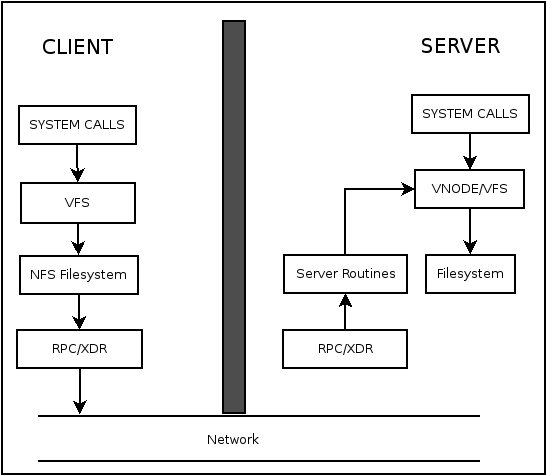
\includegraphics[width=0.5\textwidth,natwidth=400,natheight=300]{Diagram1.png}}
\caption{VFS-NFS handover .}
\label{fig}
\end{figure}
NFS by default runs in what is called server side synchronous mode. In this
mode, when the NFS client receives a write operation, it connects to the
server, requsts a write and transfers the data. Once the transfer is
;complete, the server syncs the data to its disks. After completing the sync
operation, server returns an acknowledgment message back to the client. The
issue here is that, the client has to wait till it receives the 
acknowledgment.It cannot perform any additional write to the server till the
acknowledgment arrives. This considerably slows down the system. Further,
clients are often configured to work in client side synchronous mode.
In this mode, the client is forced to write the data to the server as
soon as it receives the request. This often causes the system to crawl.

The performance of an NFS system with client and server side synchronous
mode turned on was benchmarked with client side options in /etc/fstab set as
[rw, sync, hard, intr 0 0] and the server side options  in /etc/exports set
as [rw, no-root-squash, subtree-check]. The benchmarks were conducted using
dbench utility part of Phoronix Test Suite. This resulted in performance of
0.94 MB/s. The server and client systems in this case were equipped with
100mbps network adapters. The speeds obtained are thus clearly sub-optimal.
The peformance graph obtained from the benchmark has been shown in figure.
\begin{figure}[htbp]
\centerline{\includegraphics[width=0.5\textwidth,natwidth=400,natheight=50]{nfs_working_fig_2.png}}
\caption{Performance graph.}
\label{fig}
\end{figure}

\section{Parameters affecting performance}
NFS operates on the client-server architecture. There are tweaks that can
be applied to NFS both at the client and server end. At the client end, the
tweaks are made to /etc/fstab file and at the server end, the configuration
is done to the /etc/exports file. Some of the commonly used options are listed below.
\begin{table}[htbp]
\caption{NFS Options-Client Side}
\begin{center}
\begin{tabular}{|c|c|c|}
\hline
\cline{2-3} 
\textbf{SlNo.} & \textbf{\textit{Option}}& \textbf{\textit{Description}} \\
\hline
1& rw & Read/Write  \\
2& syn & Sync file system with the server  \\
3& hard & NFS requests are retried indefinitely  \\
4& intr & Provided for backward compatibility \\
5& nfsvers & Specifies the nfs versions  \\
6& rsize & Maximum number of bytes when reading data  \\
7& wsize & Maximum number of bytes when writing data  \\
8& udp & Specifies the connection to UDP  \\
9& async & Asynchronous write  \\
\hline
\end{tabular}
\label{tab2}
\end{center}
\end{table}
\begin{table}[htbp]
\caption{NFS Options-Server Side}
\begin{center}
\begin{tabular}{|c|c|c|}
\hline
\cline{2-3} 
\textbf{SlNo.} & \textbf{\textit{Option}}& \textbf{\textit{Description}} \\
\hline
1& rw & Read/Write  \\
2& no-root-squash & Turn off root squashing  \\
3& subtree-check & Specified directory/its subrectory for access  \\
4& async & Synchronous write \\
5& sync & Asynchronous write  \\
\hline
\end{tabular}
\label{tab1}
\end{center}
\end{table}
Various compbinations of these options were benchmarked. It was found that
most of the options provided no increment in the performance of NFS
environment with performance in the ball park of 0.94 MB/s.
One notabble
exception was the client side UDP option which reduced the speeds to
0.77 MB/s. At the end of experiments, it was found that considerable 
increase in performance was provided only by client side and server side 
async.

\section{Performance with Server side ASYNC}
In server side synchronous mode, the server waits till the data has been 
written to its disk before returning the acknowledgment message to the 
client. Server side asynchronous mode changes the behaviour of NFS server 
such that it returns the acknowledgment message as soon as the client 
completes the transfer of data. This has tremendous impact on the
performance of the system.

An NFS system with server side asynchronous mode was benchmarked with the
client side options in /etc/fstab set as [rw, sync, hard, intr 0 0] and
server side options in /etc/exports set as 
[rw,no-root-squash,no-subtree-check, async]. The test was conducted using
dbench tool - part of phoronix test suite, and resulted in 28.72 MB/s, a
huge increase in performance boost, compared with the earlier server side
synchronous mode, which returned 0.94 MB/s. The performance graph obtained has been shown in figure.
\begin{figure}[htbp]
\centerline{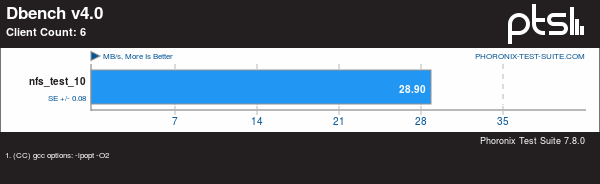
\includegraphics[width=0.5\textwidth,natwidth=400,natheight=300]{server_async_fig.png}}
\caption{Performance figure .}
\label{fig}
\end{figure}
Further benchmarks were also conducted with dd utility, with a block size
of 1KB, file size of 2GB and fdatasync option turned on. The block size of
1K ensures the computer writes only 1KB of data at a time and the fdatasync
option flushes the cache after each block is written. The aim was to
understand the performance of the system without the contribution of client
side caches. The benchmark resulted in 7.1 MB/s which was stil significantly
higher than results recorded with server side asynchronous mode.

Performance Figure

The higher performance comes from the fact that the clients do not have to 
wait till the server syncs the data with its disks. Clients can transfer
data to the server, then get on with other tasks such as writing additional
files. This also means that more number of clients can access the server
in unit time. Still, with the current protocol, it is not advisable to leave
server side async turned on due to the possibility of data loss and
corruption.
\subsection{Reliability concerns with Server side ASYNC}\label{AA}
One side effect of enabling server side asynchronous mode is that, more
clients can access the server in unit time. This in turn can cause a write
queue to form on the client side. That is, writing a file to the server
gives no guarantee that it has been written to permanent storage. In case
the server crashes immediately after some data has been transferred to it,
be it software crash or hardware failure, it can cause data corruption or 
loss. The more worrying fact is that, it is not just a single computer which
looses data. Data loss can occour to most of the clients which has written 
to the server shortly before the crash.

If a server crash occours, a client has no means of protecting itself from
the data loss. A client has no NFS cache that is permanent in nature. Even
if the client has the lost file in its primary memory, there is a high
chance of loosing it. This is because, if prior to crash the server was
serving a critical configuration file, the application dependant on the file
can crash. If the application is part of the Operating System, it can bring
down the whole system. The latter is often the case with environments where
home directory is served by an NFS share. Thus, with the current system,
server side asynchronous mode is a very risky option to leave turned on.

\subsection{Fixing server side ASYNC behaviour}

Once VFS handovers the write request to NFS client, it transfers the 
received data to the server rather than writing it to the local storage. In
case of data loss, the file cannot be recovered, as the only copy of the
file was in server's memory. The solution is to create a buffer in the 
client's local storage such that, a copy of all the data written to server 
will be kept with the client.

The buffer is a predefined storage area in the client's secondary memory.
It acts like a ring buffer with a flexible memory size. The oldest files are
deleted once the buffer reaches a predefined size. NFS client will maintain
a plaintext file in the buffer containing names of each file in the buffer,
its path and hash generated from each file. During an NFS write operation,
the client stores a copy of the file in the buffer area and updates the 
metadata file with the information regarding the  new file. The hash is
calculated whenever a file is written to the buffer. To minimize the CPU
overhead for hash calculation, a lightweight hashing algorithm such as QUARK\cite{b4}
or PHOTON\cite{b5}. Figure shows the working and structure of the buffer.
\begin{figure}[htbp]
\centerline{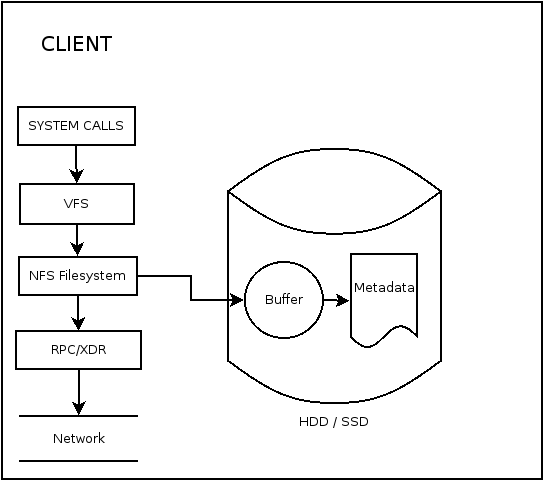
\includegraphics[width=0.5\textwidth,natwidth=400,natheight=50]{fixing_server_async.png}}
\caption{Working and structure of buffer.}
\label{fig}
\end{figure}
\begin{figure}[htbp]
\centerline{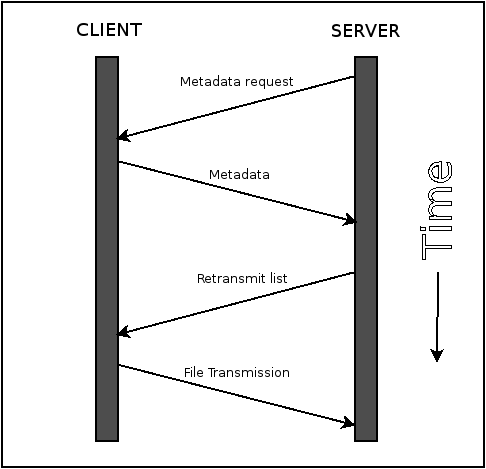
\includegraphics[width=0.5\textwidth,natwidth=400,natheight=50]{error_recovery.png}}
\caption{Working and structure of buffer.}
\label{fig}
\end{figure}


In case of a server crash, the server creates a list of corrupted or lost
files. During the first boot after the crash, the server requests the
metadata file from each client that connects to it. Once the server receives
the metadata, it calculates the hash for the local copy of each file that
is listed in the metadata. If a file is missing or if the hashes do not
match, they are added to retransmit-list, a list of files to be 
retransmitted from the client. Once the metadata file from a client is fully
scanned, the retransmit list is sent to the client. The client in turn
transmits a new copy of each file in the retransmit list. Figure shows the
error recovery process.

\subsection{Advantages of the proposed solution}
The proposed solution has a number of advantages, the most important one
being higher security against data corruption and loss. With the current 
system, server side asynchronous mode is turned off by default, due to 
concerns about data loss. The proposed solution once implemented, virtually
eliminates the chance of data loss and makes it safe to leave the server
side asynchronous mode turned on.

The solution allows the NFS environment to maintain high speeds while
keeping chances of data loss negligibly low. The solution is also easy to
implement as it requires changes to only the NFS protocol and leaves the
Operating System untouched.

\section{Client side Asynchronous mode}
Client side asynchronous mode is another method, that can be used to improve
the performance of Network File System. Client side asynchronous mode uses
the client's RAM as a giant cache. Once enabled, writes to the NFS server
are instead written to the client's RAM. The file gets written to server 
only if one of the following conditions are met:
\begin{itemize}
\item Memory fills up
\item An application flushes cache using sync, fsync or msync
\item A file is closed with close()
\item A file is locked/unlocked using fcntl
\item Client shutdown
\end{itemize}

That is, when using client side asynchronous mode, writes to the server are
drastically reduced. This benefits both the client doing the write and the
environment as a whole. For the client, it reduces the number of instances
it has to transfer data to the server. For the server, it reduces the
number of writes it has to deal with in unit time. This also means that the
rest of the clients have to wait less to read/write to the server.

The performance from client side asynchronous mode is not obvious from
benchmarks. Client side asynchronous mode has mixed results from the 
benchmarks with pts/dbench measuring a marginally low 24 MB/s down from 
28 MB/s with only server side asynchronous mode turned on, while dd 
measured 68 MB/s, an increase of 10 MB/s compared with only server side
asynchronous mode turned on. Regardless of the benchmark, client side 
asynchronous mode certainly improves the performance of the network.

\subsection{Enhancing client side ASYNC }\label{SCM}
The behaviour of client side asynchronous mode can be further enhanced to 
optimize the performance of an NFS environment. This can be done by
modifying the server such that it keeps two variables, max-count and 
current-count. max-count is the maximum number of clients which can write 
to the NFS server at a time, while current-count is the number of clients 
which are currently writing to the server. max-count is a user configurable
value and can be optimized as per the size of the network.

The client side asynchronous behaviour is modified such that, the clients 
try to write to the server as soon as a threshold is reached. The threshold
is user configurable and can be optimized as per the configuration of the
system. The server initially sets the value of current-count to 0. The 
server increments the value by one whenever a new client connects. When the
client tries to connect to the server, the server checks if the
current-count is less than max-count. The server allows the client to
connect only if max-count - current-count >= 1. In case the server has
reached its client limit, it denies the connection. The client waits for a
random time rand-wait-time before trying to connect again. rand-wait-time
is also user configurable and needs to be optimized per the size of the
network.Figure shows the propsed behaviour of client side asynchronous mode.
\begin{figure}[htbp]
\centerline{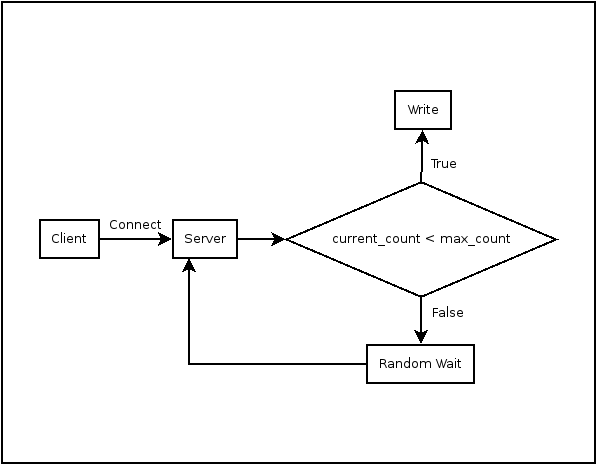
\includegraphics[width=0.5\textwidth,natwidth=400,natheight=100]{enhancing_client_async.png}}
\caption{Error recovery.}
\label{fig}
\end{figure}

\subsection{Advantages of proposed solution}
The proposed solution provides a number of considerable advantages over the
current system. First and foremost, it guards the data against corruption.
With the current system, a particular file can remain in the memory for too
long. The proposed system forces the NFS client to flush its caches when a
limit is reached. That is, a file won't remain in the cache for long, making
sure it gets written to the server and to the proposed buffer, reducing the
risk of data corruption.

The current client side asynchronous mode tries to fill up the RAM before
trying to transfer the contents to the buffer. This can negatively affect
the performance of both the applications running on the client and the
network. If a particularly heavy application needs to be loaded, the client 
is forced to flush the caches, thus initiaing the NFS write. The client
will need to wait for the write to complete before the application can be
properly loaded. This introduces unnecessary latency to the system. The 
proposed system also makes sure that server's capacity is not wasted. The 
system makes sure a healthy number of clients gets to write to the server
throughout its running time.

Regardless of the number of active clients, the number of clients doing
write to the server will remain a constant. This can improve the overall 
performance of the environment by ensuring that the server can provide 
decent read/write speeds regardless of the state of the environment. Thus
the proposed system can provide a speedy and mature NFS behaviour.
\section{Conclusion}
Network File System, though introduced in 1984, is still a widely deployed
distributed file system. The paper introduces a couple of methods which can
enhance the reliability and performance of the Network File System.

The paper proposes a pseudo ring buffer on the client's secondary storage
and proposes changes to the behaviour of NFS client and server to 
drastically reduce the rate of data corruption and loss when using server
side asynchronous mode. The paper also proposes changes in behaviour of the
NFS client and server when using client side asynchronous mode with an aim 
to reduce data loss and improve overall performance of the system.

Once implemented, the changes suggested in this paper can enhance the
performance of the NFS protocol while bringing down risk of data corruption
and loss.
\section*{References}

Please number citations consecutively within brackets \cite{b1}. The 
sentence punctuation follows the bracket \cite{b2}. Refer simply to the reference 
number, as in \cite{b3}---do not use ``Ref. \cite{b3}'' or ``reference \cite{b3}'' except at 
the beginning of a sentence: ``Reference \cite{b3} was the first $\ldots$''

Number footnotes separately in superscripts. Place the actual footnote at 
the bottom of the column in which it was cited. Do not put footnotes in the 
abstract or reference list. Use letters for table footnotes.

Unless there are six authors or more give all authors' names; do not use 
``et al.''. Papers that have not been published, even if they have been 
submitted for publication, should be cited as ``unpublished'' \cite{b4}. Papers 
that have been accepted for publication should be cited as ``in press'' \cite{b5}. 
Capitalize only the first word in a paper title, except for proper nouns and 
element symbols.

For papers published in translation journals, please give the English 
citation first, followed by the original foreign-language citation \cite{b6}.

\begin{thebibliography}{00}
\bibitem{b1} Russel Sandberg and David Gold Berg "Design and Implementation of Sun Network FIle System". 
\bibitem{b2} Athicha Muthitacharoen, Benjie Chen, and David Mazieres "A Low-bandwidth Network File System".
\bibitem{b3} Rohit Dube, Cynthia D. Rais and Satish K. Tripathi, "Improving NFS Performance over Wire Links".
\bibitem{b4} Jean-Philippe Aumasson, Luca Henzen, Willi Meier and  Marıa Naya-Plasencia, "Quark: a lightweight hash".
\bibitem{b5}Jian Guo, Thomas Peyrin and Axel Poschmann, "The PHOTON Family of Lightweight Hash Functions"

\end{thebibliography}

\end{document}
